\chapter{\diagTitle}\label{sec:diagonalization}



Given a linear transformation, it is highly desirable to write its matrix  with respect to a basis of eigenvectors.

\section{Diagonalizability}\index{Diagonalization}

Suppose we are lucky, and we have $L \colon V\to V$, and the ordered basis 
$B=(v_1, \ldots, v_n )$ is a set of %linearly independent 
eigenvectors for $L$, with eigenvalues $\lambda_1, \ldots, \lambda_n$.  Then:

\begin{eqnarray*}
L(v_1)&=&\lambda_1 v_1 \\
L(v_2)&=&\lambda_2 v_2 \\
&\vdots & \\
L(v_n)&=&\lambda_n v_n \\
\end{eqnarray*}
As a result, the matrix of $L$ in the basis of eigenvectors $B$ is diagonal:
\[
L\begin{pmatrix}
x^1\\
x^2\\
\vdots\\
x^n
\end{pmatrix}_B
=
\left(
\begin{pmatrix}
\lambda_1    \\
& \lambda_2 &  & \\
&  & \ddots &  \\
& & & \lambda_n
\end{pmatrix}
\begin{pmatrix}
x^1\\
x^2\\
\vdots\\
x^n
\end{pmatrix}
\right)_B
,
\]
where all entries off the diagonal are zero.

Suppose that \(V\) is any \(n\)-dimensional vector space. We call a linear transformation $L \colon V\mapsto V$ \emph{diagonalizable}\index{Diagonalizable} if there exists a collection of $n$ linearly independent eigenvectors for $L$.  In other words, $L$ is diagonalizable if there exists a basis for $V$ of eigenvectors for $L$.  

In a basis of eigenvectors, the matrix of a linear transformation is diagonal.  On the other hand, if an $n \times n$ matrix is diagonal, then the standard basis vectors $e_i$ must already be a set of $n$ linearly independent eigenvectors.  We have shown:

\begin{theorem}
Given an ordered basis $B$ for a vector space $V$ and a linear transformation $L \colon V\rightarrow V$, then the matrix for $L$ in the basis $B$ is diagonal if and only if $B$ consists of eigenvectors for $L$.
\end{theorem}

\Videoscriptlink{diagonalization_derivative.mp4}{Non-diagonalizable example}{scripts_diagonalization_derivative}

%\begin{center}\href{\webworkurl ReadingHomework20/2/}{Reading homework: problem 20.2}\end{center}
\Reading{Diagonalization}{1}

Typically, however, we do not begin a problem with a basis of eigenvectors, but rather have to compute these. Hence we need to know how to change from one basis to another:

\section{Change of Basis}\index{Change of basis}

Suppose we have two  ordered bases $S=(v_1, \ldots, v_n )$ and 
$S'=(v'_1, \ldots, v'_n )$ for a vector space $V$. (Here $v_i$ and $v'_i$ are {\it vectors}, not components of vectors in a basis!) 
Then we may write each $v'_k$ uniquely as 
\[
v'_k = \sum_i v_ip^i_k\, ,
\]
this is $v'_k$ as a linear combination of the~$v_i$. 
In  matrix notation
\[ 
\rowvec{v'_1 , v'_2 , \cdots , v'_n} = \rowvec{v_1 , v_2 , \cdots , v_n}
\begin{pmatrix}p^1_1&p^1_2&\cdots &p^1_n\\ p^2_1 & p^2_2 && \\[2mm]
                                              \mc\vdots &&&\mc\vdots\\ p^n_1 &&\cdots & p^n_n\end{pmatrix}\, .
\]
Here, the $p^i_k$ are constants, which we can regard as entries of  a square matrix~$P=(p^i_k)$.  The matrix~$P$ must have an inverse since we can also write each~$v_j$ uniquely as a linear combination of the~$v'_k$;
\[
v_j = \sum_k v_k' q^k_j.
\]

Then we can write
\[
v_j = \sum_k \sum_i v_ip^i_kq^k_j.
\]
But $\sum_k p^i_kq^k_j$ is the $k,j$ entry of the product matrix  $PQ$.  Since the  expression for $v_j$ in the basis $S$ is $v_j$ itself, then $PQ$ maps each  $v_j$ to itself.  As a result, each $v_j$ is an eigenvector for $PQ$ with eigenvalue $1$, so $PQ$ is the identity, {\it i.e.}
$$
PQ=I \Leftrightarrow Q=P^{-1}\, .
$$

\vspace{1mm}
The matrix $P$ is  called a \emph{change of basis} matrix\index{Change of basis matrix}. There is a quick and dirty trick to obtain it; look at the formula above relating the new basis vectors
$v'_1,v'_2,\ldots v'_n$ to the old ones $v_1,v_2,\ldots,v_n$. In particular focus on $v'_1$ for which
$$
v'_1= \begin{pmatrix}v_1 , v_2 , \cdots , v_n\end{pmatrix}
\begin{pmatrix}p^1_1\\p^2_1\\\mc\vdots \\ p^n_1
\end{pmatrix}\, .
$$
This says that the first column of the change of basis matrix $P$ is really just the components of the vector $v'_1$ in the basis $v_1,v_2,\ldots,v_n$. 

\Shabox{1}{\begin{tabular}{c}The columns of the change of basis matrix are the components\\ of the new basis vectors  in terms of the old basis vectors.\end{tabular} }

\begin{example}
Suppose  $S'=(v'_1,v'_2)$ is an ordered  basis for a vector space $V$ and that with respect to some other ordered basis $S=(v_1, v_2)$ for $V$ 
$$
v'_1=
\begin{pmatrix}
\frac{1}{\sqrt{2}}\\\frac{1}{\sqrt{2}}
\end{pmatrix} _S
\quad \mbox{and} \quad 
v'_2=
\begin{pmatrix}
\frac{1}{\sqrt{3}}\\-\frac{1}{\sqrt{3}}
\end{pmatrix}_S  \, .
$$
%What is the change of basis matrix $P$ from the old basis $u_1, u_2$ to the new basis $v_1,v_2$?
%
%Before answering note that the above 
This means 
$$
v'_1=\begin{pmatrix}v_1 , v_2 \end{pmatrix}\begin{pmatrix}
\frac{1}{\sqrt{2}}\\ \frac{1}{\sqrt{2}}
\end{pmatrix}
=\frac{v_1+v_2}{\sqrt{2}}\quad\mbox{and}\quad
v'_2=\begin{pmatrix}v_1 , v_2 \end{pmatrix}\begin{pmatrix}
\frac{1}{\sqrt{3}}\\-\frac{1}{\sqrt{3}}
\end{pmatrix}
=\frac{v_1-v_2}{\sqrt{3}}\, .
$$
The change of basis matrix has as its columns just the components of $v'_1$ and $v'_2$;
$$
P= \begin{pmatrix}
\frac{1}{\sqrt{2}}&\frac{1}{\sqrt{3}}\\
\frac{1}{\sqrt{2}}&-\frac{1}{\sqrt{3}}
\end{pmatrix}\, .
$$
\end{example}


\vspace{1mm}


Changing basis changes the matrix of a linear transformation. However, as a map between vector spaces, {\bf the linear transformation is the same no matter which basis we use}. Linear transformations are the actual objects of study of this book, not matrices; matrices are merely a convenient way of doing computations.

\Videoscriptlink{diagonalization_basis.mp4}{Change of Basis Example}{scripts_diagonalization_basis}

Lets now calculate how the matrix of a linear transformation changes when changing basis.
To wit, let $L \colon V \longrightarrow W$ with matrix $M=(m^i_j)$ in the ordered input and output bases $S=(v_1, \ldots, v_n )$ and $T=(w_1,\ldots,w_m)$ so
\[
L(v_i) = \sum_k w_km^k_i.
\]
Now, suppose $S'=(v'_1, \ldots, v'_n )$ and $T'=(w'_1,\ldots,w'_m)$ are new  ordered input and out bases with matrix $M'=({m'}_i^k)$. Then
\[
L(v'_i)= \sum_k w_km'^k_i\, .
\]
%where 
%$D$ 
%$$D = (d^i_j)=\begin{pmatrix}
%\lambda_1    \\
%& \lambda_2 &  & \\
%&  & \ddots &  \\
%& & & \lambda_n
%\end{pmatrix}\, ,$$
%is the diagonal matrix whose diagonal entries $d^k_k$ are the eigenvalues~$\lambda_k$. 
Let $P=(p^i_j)$ be the change of basis matrix from input basis $S$ to the basis $S'$ and $Q=(q^j_k)$ be the change of basis matrix from output basis $T$ to the basis $T'$.  Then:
\[
L(v'_j)=L\left(\sum_i v_i p^i_j\right) = \sum_i L(v_i)p^i_j
= \sum_i \sum_k w_k m^k_i p^i_j.
\]
Meanwhile, we have:
\[
L(v'_i) = \sum_kv_km'^k_i = \sum_k \sum_j v_j q^j_km^k_i.
\]
Since the expression for a vector in a basis is unique, then we see that the entries of $MP$ are the same as the entries of $QM'$.  In other words, we see that
\Shabox{1.1}{
$
MP = QM' \qquad \text{or}\qquad M'=Q^{-1}MP.
$}

\begin{example}
Let $V$ be the space of polynomials in $t$ and degree 2 or less and $\sloppy{L:V\to {\mathbb R}^2}$ where
$$
L(1)=\colvec{1\\2}\, \quad L(t)=\colvec{2\\1}\, ,\quad L(t^2)=\colvec{3\\3}\, .
$$
From this information we can immediately read off the matrix~$M$ of $L$ in the bases $S=(1,t,t^2)$ and $T=(e_1,e_2)$, the standard basis for ${\mathbb R}^2$,
because
\begin{eqnarray*}\big(L(1),L(t),L(t^2)\big)&=&(e_1+2 e_2,2e_1+e_2, 3 e_1+3e_2)\\[2mm]&=&(e_1,e_2)\begin{pmatrix}1&2&3\\2&1&3\end{pmatrix}\, \Rightarrow \, M\ =\ 
\begin{pmatrix}1&2&3\\2&1&3\end{pmatrix}\, .\end{eqnarray*}
Now suppose we are more interested in the bases $$S'=(1+t,t+t^2,1+t^2)\, , \quad T'=\left(\colvec{1\\2},\colvec{2\\1}\right)=:(w_1',w_2')\, .$$
To compute the new matrix $M'$ of $L$ we could simply calculate what $L$ does the the new input basis vectors in terms of the new output basis vectors:
\begin{eqnarray*}
\big(L(1+t),L(t+t^2),L(1+t^2))&=&\left(\colvec{1\\2}+\colvec{2\\1},
\colvec{2\\1}+\colvec{3\\3},\colvec{1\\2}+\colvec{3\\3}
\right)\\[2mm]
&=&(w'_1+w'_2,w'_1+2w'_2,2w'_1+w'_2)\\[2mm]&=&(w'_1,w'_2)
\begin{pmatrix}1&1&2\\1&2&1\end{pmatrix}\, \Rightarrow \, 
M'=\begin{pmatrix}1&1&2\\1&2&1\end{pmatrix}\, .
\end{eqnarray*}
Alternatively we could calculate the change of basis matrices $P$ and $Q$ by noting that
$$
(1+t,t+t^2,1+t^2)=(1,t,t^2)\begin{pmatrix}1&0&1\\1&1&0\\0&1&1\end{pmatrix}\, \Rightarrow\, P=\begin{pmatrix}1&0&1\\1&1&0\\0&1&1\end{pmatrix}
$$
and
$$
(w'_1,w'_2)=(e_1+2e_2,2e_1+e_2)=(e_1,e_1)\begin{pmatrix}1&2\\2&1\end{pmatrix}\, \Rightarrow\, Q=\begin{pmatrix}1&2\\2&1\end{pmatrix}\, .
$$
Hence
$$
M'=Q^{-1}MP = -\frac{1}{3}\begin{pmatrix}1&-2\\-2&1\end{pmatrix}\begin{pmatrix}1&2&3\\2&1&3\end{pmatrix}
\begin{pmatrix}1&0&1\\1&1&0\\0&1&1\end{pmatrix}=\begin{pmatrix}1&1&2\\1&2&1\end{pmatrix}\, .
$$
Notice that the change of basis matrices $P$ and $Q$ are both square and invertible. Also, since we really wanted $Q^{-1}$, 
it is more efficient to try and write $(e_1,e_2)$ in terms of $(w'_1,w'_2)$ which would yield directly $Q^{-1}$. Alternatively, one can check that
$MP=QM'$.
\end{example}

\section{Changing to a Basis of Eigenvectors}

If we are changing to a basis of eigenvectors, then there are various simplifications:
\begin{itemize}
\item Since $L:V\to V$, most likely you already know the matrix~$M$ of $L$ using the same input basis as output basis $S=(u_1,\ldots ,u_n)$ (say).
\item In the new basis of eigenvectors $S'(v_1,\ldots,v_n)$, the matrix~$D$ of $L$ is diagonal because $Lv_i=\lambda_i v_i$ and so
$$
\big(L(v_1),L(v_2),\ldots,L(v_n)\big)=(v_1,v_2,\ldots, v_n)
\begin{pmatrix}
\lambda_1&\mc0&\cdots&\mc0\\
\mc0&\lambda_2&&\mc0\\
\mc\vdots&&\ddots&\mc\vdots \\
\mc0&\mc0&\cdots&\lambda_n\end{pmatrix}\, .
$$
\item If $P$ is the change of basis matrix from $S$ to $S'$, the diagonal matrix of eigenvalues~$D$ and the original matrix are related by
\Shabox{1.1}{$D=P^{-1}MP$}
\end{itemize}

This motivates the following definition:
\begin{definition}
A matrix $M$ is {\bf diagonalizable} if there exists an invertible matrix $P$ and a diagonal matrix $D$ such that 
\[
D=P^{-1}MP.
\]
\end{definition}

We can summarize as follows.
\begin{itemize}
\item Change of basis rearranges the components of a vector by the change of basis matrix $P$, to give components in the new basis.
\item To get the matrix of a linear transformation in the new basis, we \emph{conjugate}\index{Conjugation} the matrix of $L$ by the change of basis matrix: $M\mapsto P^{-1}MP$.
\end{itemize}

If for two matrices $N$ and $M$ there exists a matrix $P$ such that $M=P^{-1}NP$, then we say that $M$ and $N$ are {\bf similar}\index{Similar matrices}.  Then the above discussion shows that diagonalizable matrices are similar to diagonal matrices.

\begin{corollary}
A square matrix $M$ is diagonalizable if and only if there exists a basis of eigenvectors for $M$. Moreover, these eigenvectors are the columns of a change of basis matrix \(P\) which diagonalizes \(M\).
\end{corollary}

%\href{\webworkurl ReadingHomework20/3/}{Reading homework: problem 20.3}
\Reading{Diagonalization}{2}

\begin{example}
Let's try to diagonalize the matrix
\[M=\begin{pmatrix}
-14 & -28 & -44 \\
-7 & -14 & -23 \\
9 & 18 & 29 \\
\end{pmatrix}.\]
The eigenvalues of \(M\) are determined by \[\det(M-\lambda I)=-\lambda^3+\lambda^2+2\lambda=0.\]
So the eigenvalues of \(M\) are \(-1,0,\) and \(2\), and associated eigenvectors turn out to be 
$$
v_1=\colvec{-8 \\ -1 \\ 3},~~ v_2=\colvec{-2 \\ 1 \\ 0}, {\rm ~and~~} v_3=\colvec{-1 \\ -1 \\ 1}.
$$ 
In order for \(M\) to be diagonalizable, we need the vectors \(v_1, v_2, v_3\) to be linearly independent. Notice that the matrix
\[P=\rowvec{v_1 & v_2 & v_3}=\begin{pmatrix}
-8 & -2 & -1 \\
-1 & 1 & -1 \\
3 & 0 & 1 \\
\end{pmatrix}\]
is invertible because its determinant is \(-1\). Therefore, the eigenvectors of \(M\) form a basis of \(\Re\), and so \(M\) is diagonalizable. 
Moreover, because the columns of $P$ are the components of eigenvectors, 
$$
MP=\rowvec{Mv_1 &Mv_2& Mv_3}=\rowvec{-1.v_1&0.v_2&2.v_3}=\rowvec{v_1& v_2 & v_3}\begin{pmatrix}
-1 & 0 & 0 \\
0 & 0 & 0 \\
0 & 0 & 2 \\
\end{pmatrix}\, .
$$
Hence, the matrix \(P\) of eigenvectors is a change of basis matrix that diagonalizes~\(M\);
\[P^{-1}MP=\begin{pmatrix}
-1 & 0 & 0 \\
0 & 0 & 0 \\
0 & 0 & 2 \\
\end{pmatrix}.\]
\end{example}

\Videoscriptlink{diagonalization_example.mp4}{$2\times2$ Example}{scripts_diagonalization_example}

\begin{figure}
\begin{center}
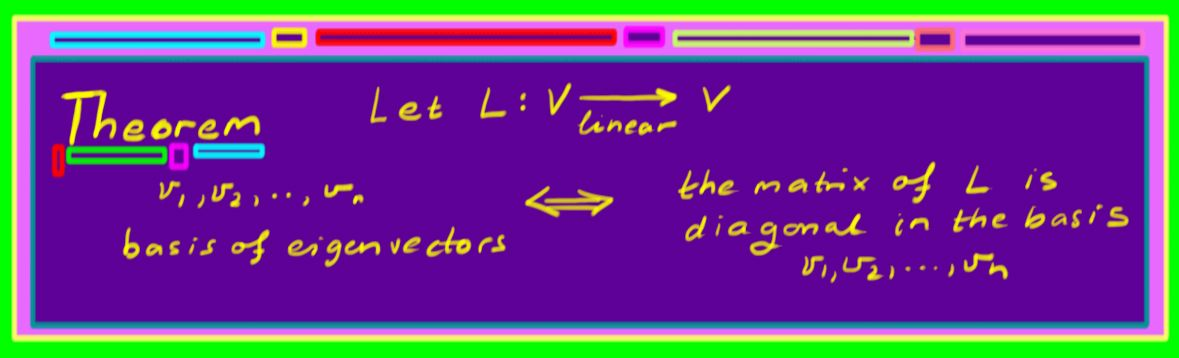
\includegraphics[scale=.33]{\diagPath/eigenbasis.jpg}
\end{center}
\caption{This theorem answers the question: ``What is diagonalization?''}
\end{figure}

%\section*{References}
%Hefferon, Chapter Three, Section V: Change of Basis
%\\
%Beezer, Chapter E, Section SD
%\\
%Beezer, Chapter R, Sections MR-CB
%\\
%Wikipedia:
%\begin{itemize}
%\item \href{http://en.wikipedia.org/wiki/Change_of_basis}{Change of Basis}
%\item \href{http://en.wikipedia.org/wiki/Diagonalizable_matrix}{Diagonalizable Matrix}
%\item \href{http://en.wikipedia.org/wiki/Similar_matrix}{Similar Matrix}
%\end{itemize}
%

\section{Review Problems}

{\bf Webwork:} 
\begin{tabular}{|c|c|}
\hline
Reading Problems & 
 \hwrref{Diagonalization}{1}, \hwrref{Diagonalization}{2}\\
No real eigenvalues &  \hwref{Diagonalization}{3}\\
Diagonalization &  \hwref{Diagonalization}{4}, \hwref{Diagonalization}{5},  \hwref{Diagonalization}{6},
 \hwref{Diagonalization}{7}\\
  \hline
\end{tabular}





\begin{enumerate}

\item While performing  Gaussian elimination on these augmented matrices write the full system of equations describing the new rows in terms of the old rows above each equivalence symbol as in  \hyperlink{Keeping track of EROs with equations between rows}{Example}~\ref{Rsystem}. 
$$
\begin{amatrix}{2} 
2 & 2 & 10 \\
1 & 2 & 8 \\
\end{amatrix}
,~
\begin{amatrix}{3} 
1 & 1 & 0 & 5 \\
1 & 1 & \!\!-1& 11 \\
-1 & 1 & 1 & -5 \\ 
\end{amatrix}
$$

%%%%%%%%%%%%%%%%%%%

\item Solve the vector equation by applying ERO matrices to each side of the equation to perform elimination. Show each matrix explicitly as in \hyperlink{Undoing}{Example~\ref{slowly}}.

\begin{eqnarray*}
\begin{pmatrix}
3	&6 	&2 \\ %-3
5 	&9 	&4 \\ %1
2	&4	&2 \\ %0
\end{pmatrix} 
\begin{pmatrix}
 x \\ 
y \\
z 
\end{pmatrix} 
=
\begin{pmatrix}
-3 \\ 
1  \\
0  \\
\end{pmatrix} 
\end{eqnarray*}

%%%%%%%%%%%%%%%%%%%

\item Solve this vector equation by finding the inverse of the matrix through $(M|I)\sim (I|M^{-1})$ and then applying $M^{-1}$ to both sides of the equation. 
\begin{eqnarray*}
\begin{pmatrix}
2	&1 	&1 \\ %9
1 	&1 	&1 \\ %6
1	&1	&2 \\ %7
\end{pmatrix} 
\begin{pmatrix}
 x \\ 
y \\
z 
\end{pmatrix} 
=
\begin{pmatrix}
9 \\ 
6  \\
7  \\
\end{pmatrix} 
\end{eqnarray*}


%%%%%%%%%%%%%%%%%%%

\item Follow the method of  \hyperlink{elldeeeww}{Examples~\ref{factorize} and~\ref{factorizes}} to find the $LU$ and $LDU$ factorization of 
\begin{eqnarray*}
\begin{pmatrix}
3	&3 	&6 \\ %0 %2
3 	&5 	&2 \\ %1 %1
6	&2	&5 \\ %0 %1
\end{pmatrix} .
\end{eqnarray*}



%%%%%%%%%%%%%%%%%%%%

\item 
Multiple matrix equations with the same matrix can be solved simultaneously. 
\begin{enumerate}
\item Solve both systems by performing elimination on just one augmented matrix.
\begin{eqnarray*}
\begin{pmatrix}
2	&-1 	&-1 \\ %0 %2
-1 	&1 	&1 \\ %1 %1
1	&-1	&0 \\ %0 %1
\end{pmatrix} 
\begin{pmatrix}
 x \\ 
y \\
z 
\end{pmatrix} 
=
\begin{pmatrix}
0\\ 
1  \\
0  \\
\end{pmatrix} 
,~
\begin{pmatrix}
2	&-1 	&-1 \\ %0 %2
-1 	&1 	&1 \\ %1 %1
1	&-1	&0 \\ %0 %1
\end{pmatrix} 
\begin{pmatrix}
 a \\ 
b \\
c 
\end{pmatrix} 
=
\begin{pmatrix}
2\\ 
1  \\
1  \\
\end{pmatrix} 
\end{eqnarray*}
\item Give an interpretation of the columns of $M^{-1}$ in $(M|I)\sim (I|M^{-1})$ in terms of solutions to certain systems of linear equations.
\end{enumerate}

%%%%%%%%%%%%%%%%%%%%%%%%

\item How can you convince your fellow students to never make this mistake?
\begin{eqnarray*}
\begin{amatrix}{3} 
1 & 0 & 2 & 3 \\ 
0 & 1 & 2& 3 \\
2 & 0 & 1 & 4 \\
\end{amatrix} 
& 
\stackrel{R_1'=R_1+R_2}{
\stackrel{R_2'=R_1-R_2}{ 
\stackrel{\ R_3'= R_1+2R_2}{\sim}}}
&
\begin{amatrix}{3} 
1 & 1 & 4 & 6 \\
1 & \!\!-1 & 0& 0 \\
1 & 2 & 6 & 9 
\end{amatrix}
\end{eqnarray*}

\item Is $LU$ factorization of a matrix unique?  Justify your answer.


\item[$\infty$.] If you randomly create a matrix by picking numbers out of the blue, it will probably be difficult to perform elimination or factorization; fractions and large numbers will probably be involved. To invent simple problems it is better to start with a simple answer:
\begin{enumerate}
\item Start with any augmented matrix in RREF. Perform EROs to make most of the components non-zero. Write the result on a separate piece of paper and give it to your friend. Ask that friend to find RREF of the augmented matrix you gave them. Make sure they get the same augmented matrix you started with.  
\item Create  an upper triangular matrix $U$ and a lower triangular matrix~$L$ with only $1$s on the diagonal. Give the result to a friend to factor into $LU$ form. 
\item Do the same with an $LDU$ factorization. 
\end{enumerate}
\end{enumerate}

\phantomnewpage



\newpage

